\section{Simulation et tests}

Il n'y avait pas de simulation à faire dans ce laboratoire. Cependant, des tests ont été effectués tout au long du laboratoire. De plus, le contrôle du fonctionnement de l'application avait été validé auprès de l'assistant avant la période de confinement. Je note tout de même ici les tests qui ont été effectués par moi-même afin de m'assurer du bon fonctionnement de l'application : \\\\
J'ai donc commencé par le plus simple. Tous les switchs down et un appui sur key 0 suivi d'un appui sur key 1 : \\\\
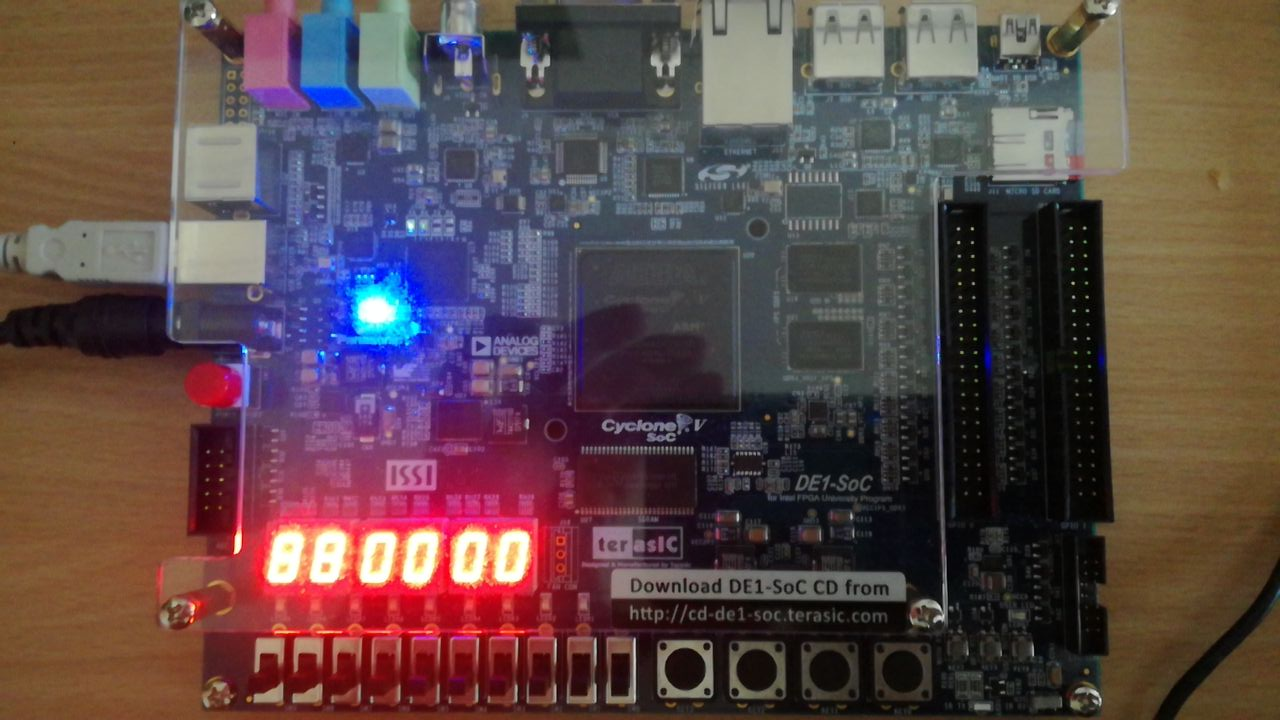
\includegraphics[scale=0.3]{./images/appuiKey0SwitchDown.jpeg}
\captionof{figure}{Laboratoire 2 : Appui key 0 avec switch down}
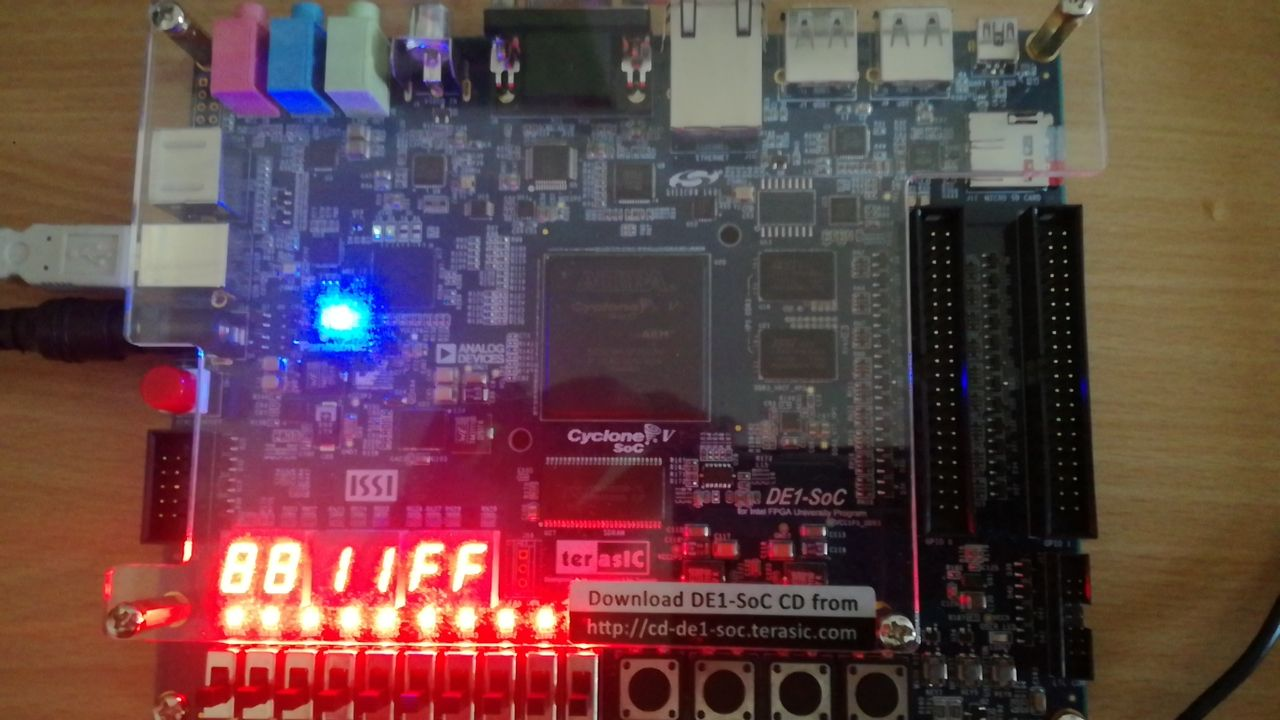
\includegraphics[scale=0.3]{./images/appuiKey1SwitchDown.jpeg}
\captionof{figure}{Laboratoire 2 : Appui key 1 avec switch down}

J'ai ensuite continué en alternant un switch down et un switch up en commençant par activer le switch 0, et j'ai appuyé sur key 0 puis sur key 1 : \\\\
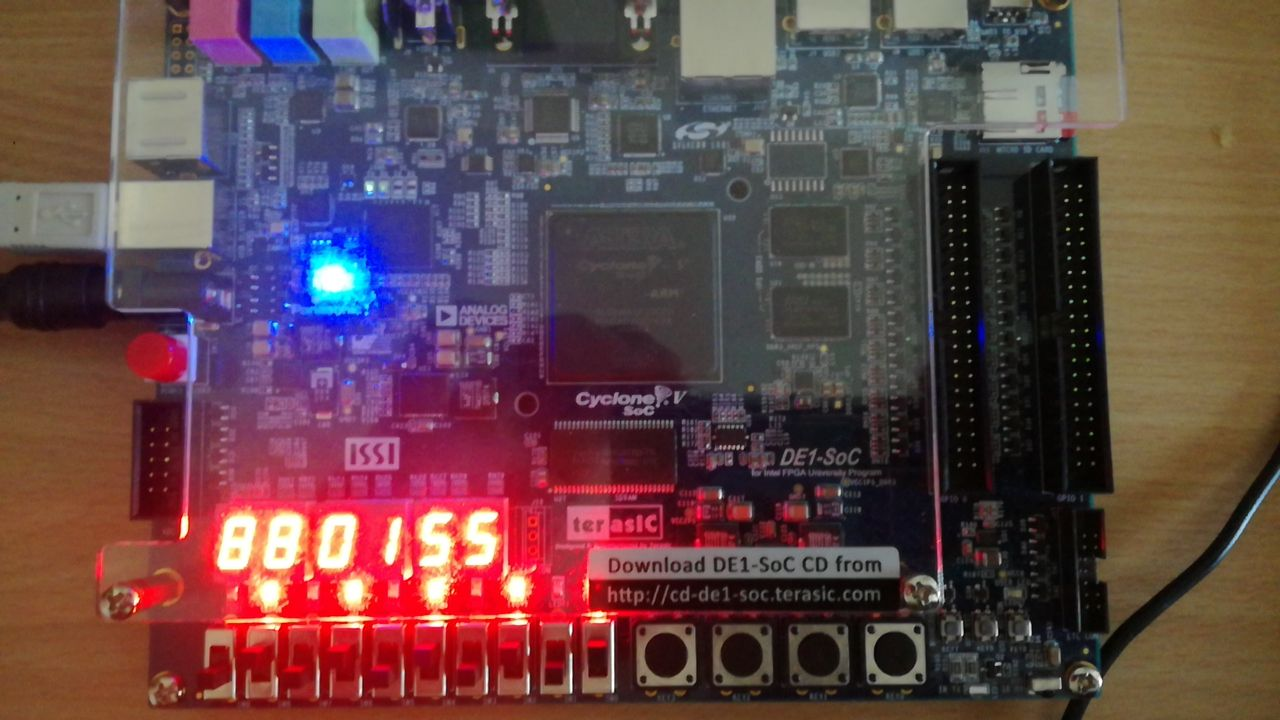
\includegraphics[scale=0.3]{./images/appuiKey0SwitchUp.jpeg}
\captionof{figure}{Laboratoire 2 : Appui key 0 avec switch up/down}
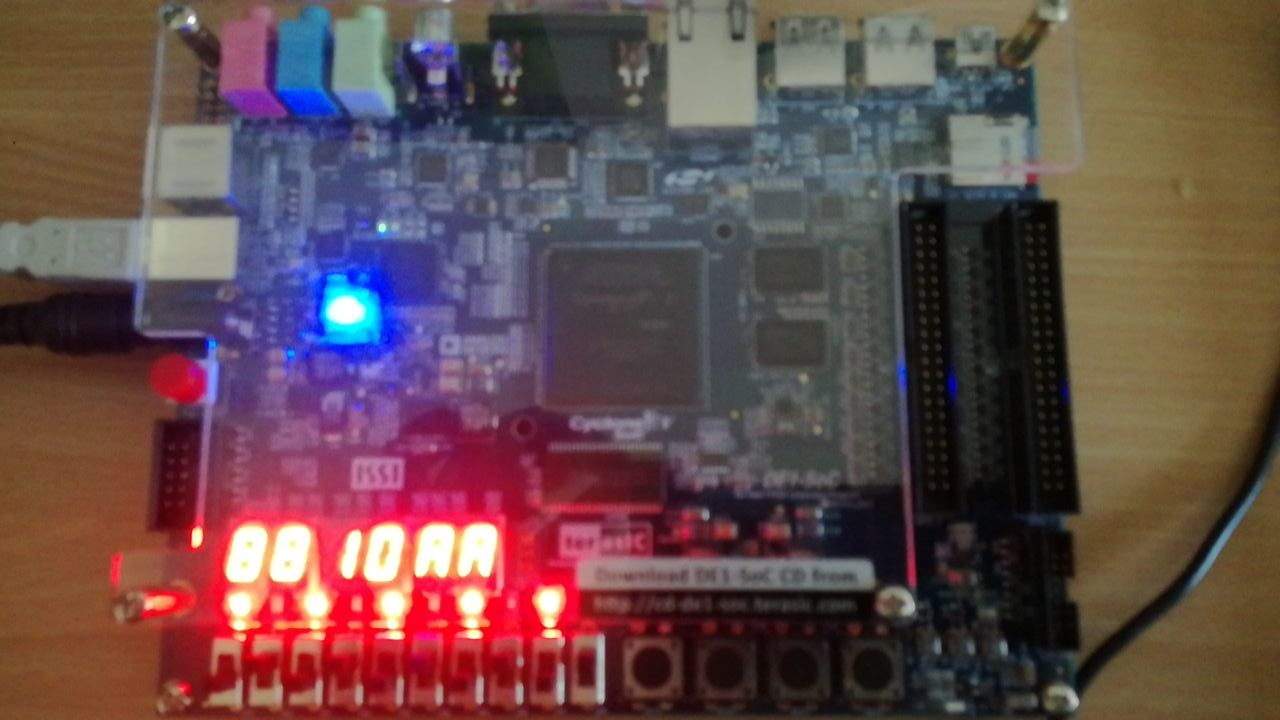
\includegraphics[scale=0.3]{./images/appuiKey1SwitchUp.jpeg}
\captionof{figure}{Laboratoire 2 : Appui key 1 avec switch up/down}

Les valeurs correspondaient au fonctionnement demandé par la donnée. Toujours avec cet état de switch, j'ai essayé les interruptions en appuyant deux fois sur key 3 puis une fois sur key 2\\\\
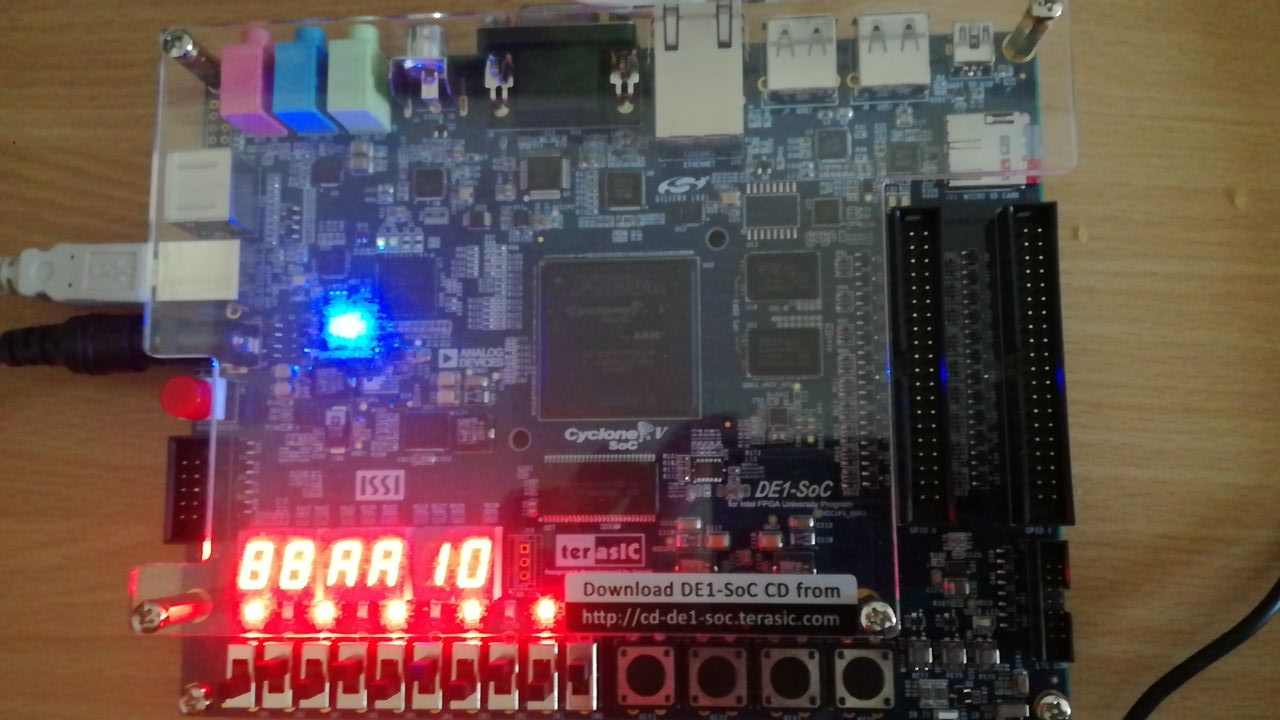
\includegraphics[scale=0.3]{./images/appuiKey3.jpeg}
\captionof{figure}{Laboratoire 2 : Appui 2 fois sur key 3}
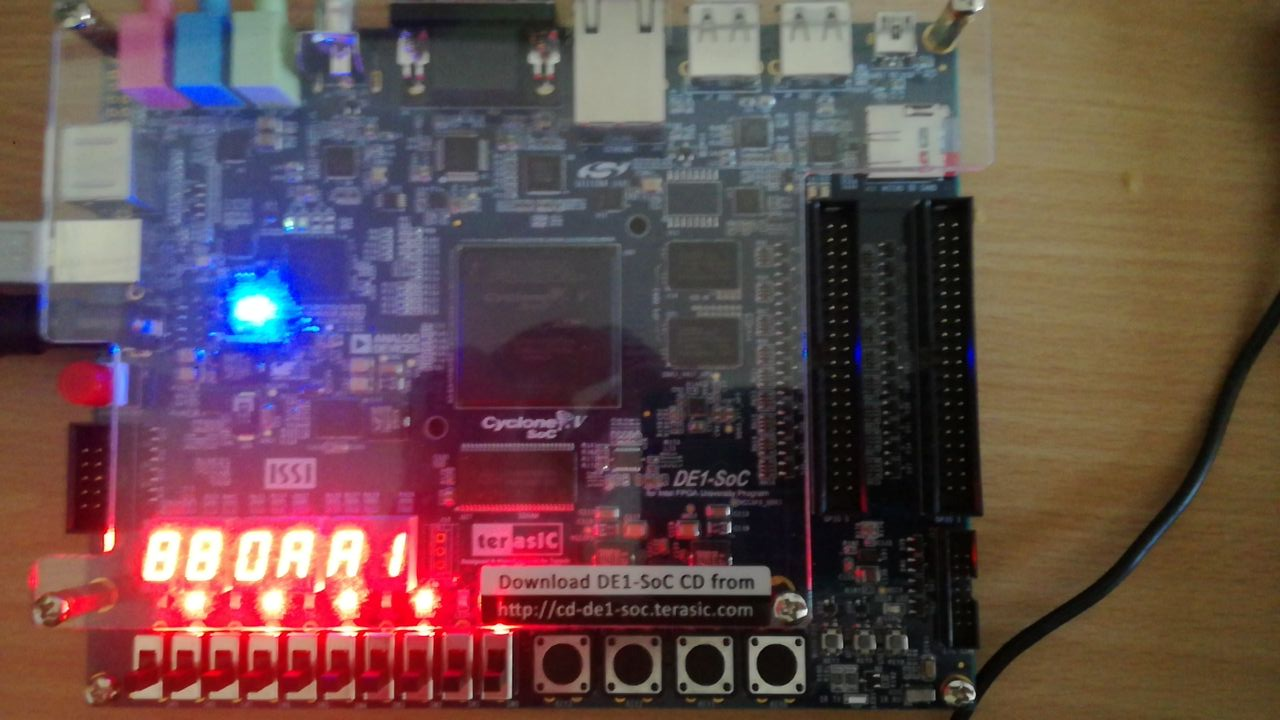
\includegraphics[scale=0.3]{./images/appuiKey2.jpeg}
\captionof{figure}{Laboratoire 2 : Appui 1 fois sur key 2}

Tout à fonctionner sans problème. J'ai testé la modification des switchs lorsque j'appuie sur key 2 ou key 3 et conformément à la donnée, les leds et l'afficheur 7 segment n'était pas impacté.